\normalfalse \difficiletrue \tdifficilefalse
\correctionfalse

%\UPSTIidClasse{11} % 11 sup, 12 spé
%\newcommand{\UPSTIidClasse}{12}

\exer{Mouvement RR 3D  $\star\star$ \label{C2:08:08}}
\setcounter{numques}{0}
\UPSTIcompetence[2]{C2-08}
\UPSTIcompetence[2]{C2-09}
\index{Compétence C2-08}
\index{Compétence C2-09}
\index{Torseur cinétique}
\index{Torseur dynamique}
\index{Mécanisme à 2 rotations 3D}
\ifcorrection
\else
\textbf{Pas de corrigé pour cet exercice.}
\fi

\ifprof
\else
Soit le mécanisme suivant. On a $\vect{AB}=H\vect{j_1}+R\vect{i_1}$ et $\vect{BC}=L\vect{i_2}$. On a $H=\SI{20}{mm}$, $r=\SI{5}{mm}$, $L=\SI{10}{mm}$. De plus :
\begin{itemize}
\item $G_1$ désigne le centre d'inertie de \textbf{1} tel que $\vect{AG_1}=H\vect{j_1}$, on note $m_1$ la masse de \textbf{1} et $\inertie{G_1}{1}=\matinertie{A_1}{B_1}{C_1}{0}{0}{0}{\bas{1}}$; 
\item $G_2=C$ désigne le centre d'inertie de \textbf{2}, on note $m_2$ la masse de \textbf{2} et $\inertie{G_2}{2}=\matinertie{A_2}{B_2}{C_2}{0}{0}{0}{\bas{2}}$.
\end{itemize}
\begin{center}
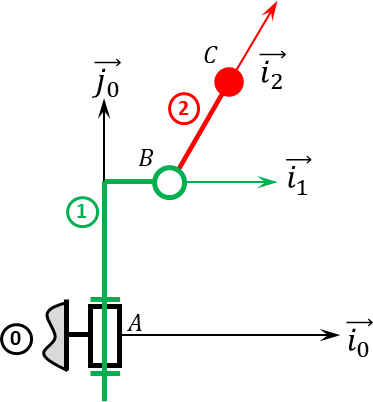
\includegraphics[width=\linewidth]{08_RR3D_01}
\end{center}

On donne : 
$\vectv{C}{2}{0} = -R\dot{\theta}\vk{1}+L\left(-\dot{\theta}\cos\varphi\vk{1} + \dot{\varphi}\vj{2}\right)$.

\textbf{On fait l'hypothèse que $\thetap$ et $\varphip$ sont des constantes et on a }

$\vectg{C}{2}{0} $
$ =L\dot{\varphi}\left(\thetap\sin\varphi\vk{1}-\varphip\vi{2}\right)
-\thetap\left( R \thetap\vi{1} +L\cos\varphi \thetap\vi{1}
-L\varphip\sin\varphi\vk{1}\right)
$.





\fi

\question{Exprimer le torseur dynamique $\torseurdyn{2}{0}$ en~$B$.}
\ifprof


Par définition, $\torseurdyn{2}{0} = \torseurl{\vectrd{2}{0}}{\vectmd{B}{2}{0}}{B}$.

\textbf{Calculons $\vectrd{2}{0}$ : } 
$\vectrd{2}{0} = m_2\vectg{G_2}{2}{0}=m_2 \vectg{C}{2}{0} $

\textbf{Calcul de $\vectv{C}{2}{0}$ : }  

$\vectv{C}{2}{0}$ 
$=\deriv{\vect{AC}}{\rep{0}}$
$=\deriv{H\vect{j_1}+R\vect{i_1}+L\vect{i_2}}{\rep{0}}$.

Calculons : 
\begin{itemize}
\item $\deriv{\vj{0}}{\rep{0}}$ $=\vect{0}$;
\item $\deriv{\vi{1}}{\rep{0}}$ $=\vecto{1}{0} \wedge \vi{1}$ $=\dot{\theta}\vj{1} \wedge \vi{1}$ $=-\dot{\theta}\vk{1}$;
\item $\deriv{\vi{2}}{\rep{0}}$ $=\vecto{2}{0} \wedge \vi{2}$ 
$=\left(\dot{\theta}\vj{1} + \dot{\varphi}\vk{2}\right)\wedge \vi{2}$
$=\dot{\theta}\vj{1}\wedge \vi{2} + \dot{\varphi}\vk{2}\wedge \vi{2}$
$=-\dot{\theta}\cos\varphi\vk{1} + \dot{\varphi}\vj{2}$.
\end{itemize}

On a donc 
$\vectv{C}{2}{0}$ 
$= -R\dot{\theta}\vk{1}+L\left(-\dot{\theta}\cos\varphi\vk{1} + \dot{\varphi}\vj{2}\right)$.

\textbf{Calcul de $\vectg{C}{2}{0}$ : }  

$\vectg{C}{2}{0} =\deriv{\vectv{C}{2}{0}}{\rep{0}}$

$ =\deriv{ L\dot{\varphi}\vj{2}-\thetap\left( R\vk{1}+L\cos\varphi\vk{1}\right)}{\rep{0}} $.

Calculons :
\begin{itemize}
\item $\deriv{\vj{2}}{\rep{0}}=\vecto{2}{0}\wedge\vj{2}$ 
$=\left(\thetap\vj{1}+\varphip\vk{1} \right)\wedge\vj{2}$ 
$=\thetap\vj{1}\wedge\vj{2}+\varphip\vk{1} \wedge\vj{2}$
$=\thetap\sin\varphi\vk{1}-\varphip\vi{2} $.
\item $\deriv{\vk{1}}{\rep{0}} = \thetap\vi{1}$.
\end{itemize}


Avec les hypothèses, on a $\vectg{C}{2}{0} $
$ =L\dot{\varphi}\left(\thetap\sin\varphi\vk{1}-\varphip\vi{2}\right)
-\thetap\left( R \thetap\vi{1} +L\cos\varphi \thetap\vi{1}
-L\varphip\sin\varphi\vk{1}\right)
$.



\vspace{.5cm}

\textbf{Calculons $\vectmd{C}{2}{0}$}

$C$ est le centre d'inertie du solide 2; donc 
d'une part, $\vectmd{C}{2}{0} = \deriv{\vectmc{C}{2}{0} }{\rep{0}}$.

 D'autre part, $\vectmc{C}{2}{0} = \inertie{C}{2}\vecto{2}{0}$. 
 
 Or $\vecto{2}{0} = \thetap \vj{1} + \varphip\vk{2}$ $= \thetap \left(\cos\varphi \vj{2} + \sin\varphi \vi{2}\right) + \varphip\vk{2}$.
 
$\vectmc{C}{2}{0} = \matinertie{A_2}{B_2}{C_2}{0}{0}{0}{\bas{2}} 
 \begin{pmatrix} 
 \thetap \sin\varphi  \\
  \thetap \cos\varphi  \\
  \varphip
 \end{pmatrix}_{\bas{2}}$
 $ =  \begin{pmatrix} 
 \thetap A_2 \sin\varphi  \\
  \thetap B_2 \cos\varphi  \\
  C_ 2 \varphip
 \end{pmatrix}_{\bas{2}}$.
%  $ =C_1 \thetap \vk{0}$.
%  
%  Par suite, $\vectmd{B}{1}{0} = C_1 \thetapp \vk{0}$.
%  
%  Au final, 
%$\torseurdyn{1}{0} = \torseurl{m_1\left(R\thetapp \vj{1}-R\thetap^2 \vi{1}\right)}{C_1 \thetapp \vk{0}}{B}$


\else
\fi

\question{Déterminer $\vectmd{A}{1+2}{0}\cdot \vect{j_0}$}
\ifprof


\else
\fi

\ifprof
\else
\begin{flushright}
\footnotesize{Corrigé  voir \ref{C2:08:08}.}
\end{flushright}%
\fi